\chapter{Úvod}

Tato práce se zaměřuje na ovládání barevného TFT displeje, připojeného k~vývojovému kitu ESP32, přes rozhraní WiFi nebo Bluetooth. Jelikož zadání povoluje výběr mezi komunikací přes WiFi a Bluetooth, pro tento projekt byla zvolena komunikace přes Bluetooth z~důvodu jednoduchého párování a přímočaré komunikaci mezi dvěma zařízeními. Avšak v~kapitole \ref{sec:test} je zmíněna i negativní stránka připojení přes Bluetooth, a to je nízký objem dat na paket, který zařízení přijímá. Ovládání je demonstrováno na možnosti vypsání textu na displej, vykreslení přijatého obrázku, nebo na možnosti hraní Tetrisu.

Veškerou funkcionalitu demonstruje následující video: \url{https://youtu.be/RHHq2XagPnQ}

\chapter{Návrh}

V~této kapitole je popsán návrh celého projektu od hardwarové části až po samotný kód. Cílem návrhu bylo vytvořit projekt, který umožní ovládání TFT displeje skrze rozhraní WiFi nebo Bluetooth, přičemž v~tomto projektu byla zvolena komunikace přes Bluetooth z~důvodu její přímočaré komunikace mezi dvěma zařízeními. Návrh v~sobě zahrnuje způsob ovládání výsledného projektu a toho je docíleno pomocí externí aplikace \cite{AppPixelBluetoothCanvas}.

\section{Hardware}

V~projektu je použit vývojový kit ESP32 Wemos D1 R32, který přes SPI rozhraní komunikuje s~1,44''~$128\times128$ TFT displejem s~označením ILI9163C.
Pro komunikaci s~počítačem nebo jiným zařízení s~podporou Bluetooth projekt využívá Bluetooth čip, který je součástí vývojového kitu, a tudíž nemusí být externě dodán.

\section{Schéma zapojení}

Na obrázku \ref{fig:zapojeni} je vyfocené zapojení TFT displeje k~vývojovému kitu ESP32. Podrobněji je zapojení jednotlivých pinů v~tabulce \ref{tab:esp32_tft_piny}. Jedná se o~komunikaci přes SPI rozhraní kde ESP32 je \textit{master} a TFT displej je \textit{slave}.

\begin{table}[h!]
    \centering
    \begin{tabular}{|c|c|c|}
        \hline
        \textbf{ESP32 pin}  & \textbf{TFT pin} & \textbf{Popis} \\
        \hline
        3.3V                & VCC              & Napájení 3.3V \\
        \hline
        3.3V                & LED              & Podsvícení displeje \\
        \hline
        GND                 & GND              & Zem \\
        \hline
        IO23                & SDA              & Master Out Slave In (SPI data) \\
        \hline
        IO18                & SCK              & SPI hodiny \\
        \hline
        IO5                 & CS               & Chip Select  \\
        \hline
        IO2                 & DC               & Data/Command \\
        \hline
        IO27                & RST              & Reset displeje \\
        \hline
    \end{tabular}
    \caption{Zapojení jednotlivých pinů vývojového kitu ESP32 na piny TFT displeje.}
    \label{tab:esp32_tft_piny}
\end{table}

\begin{figure}[h!]
    \centering
    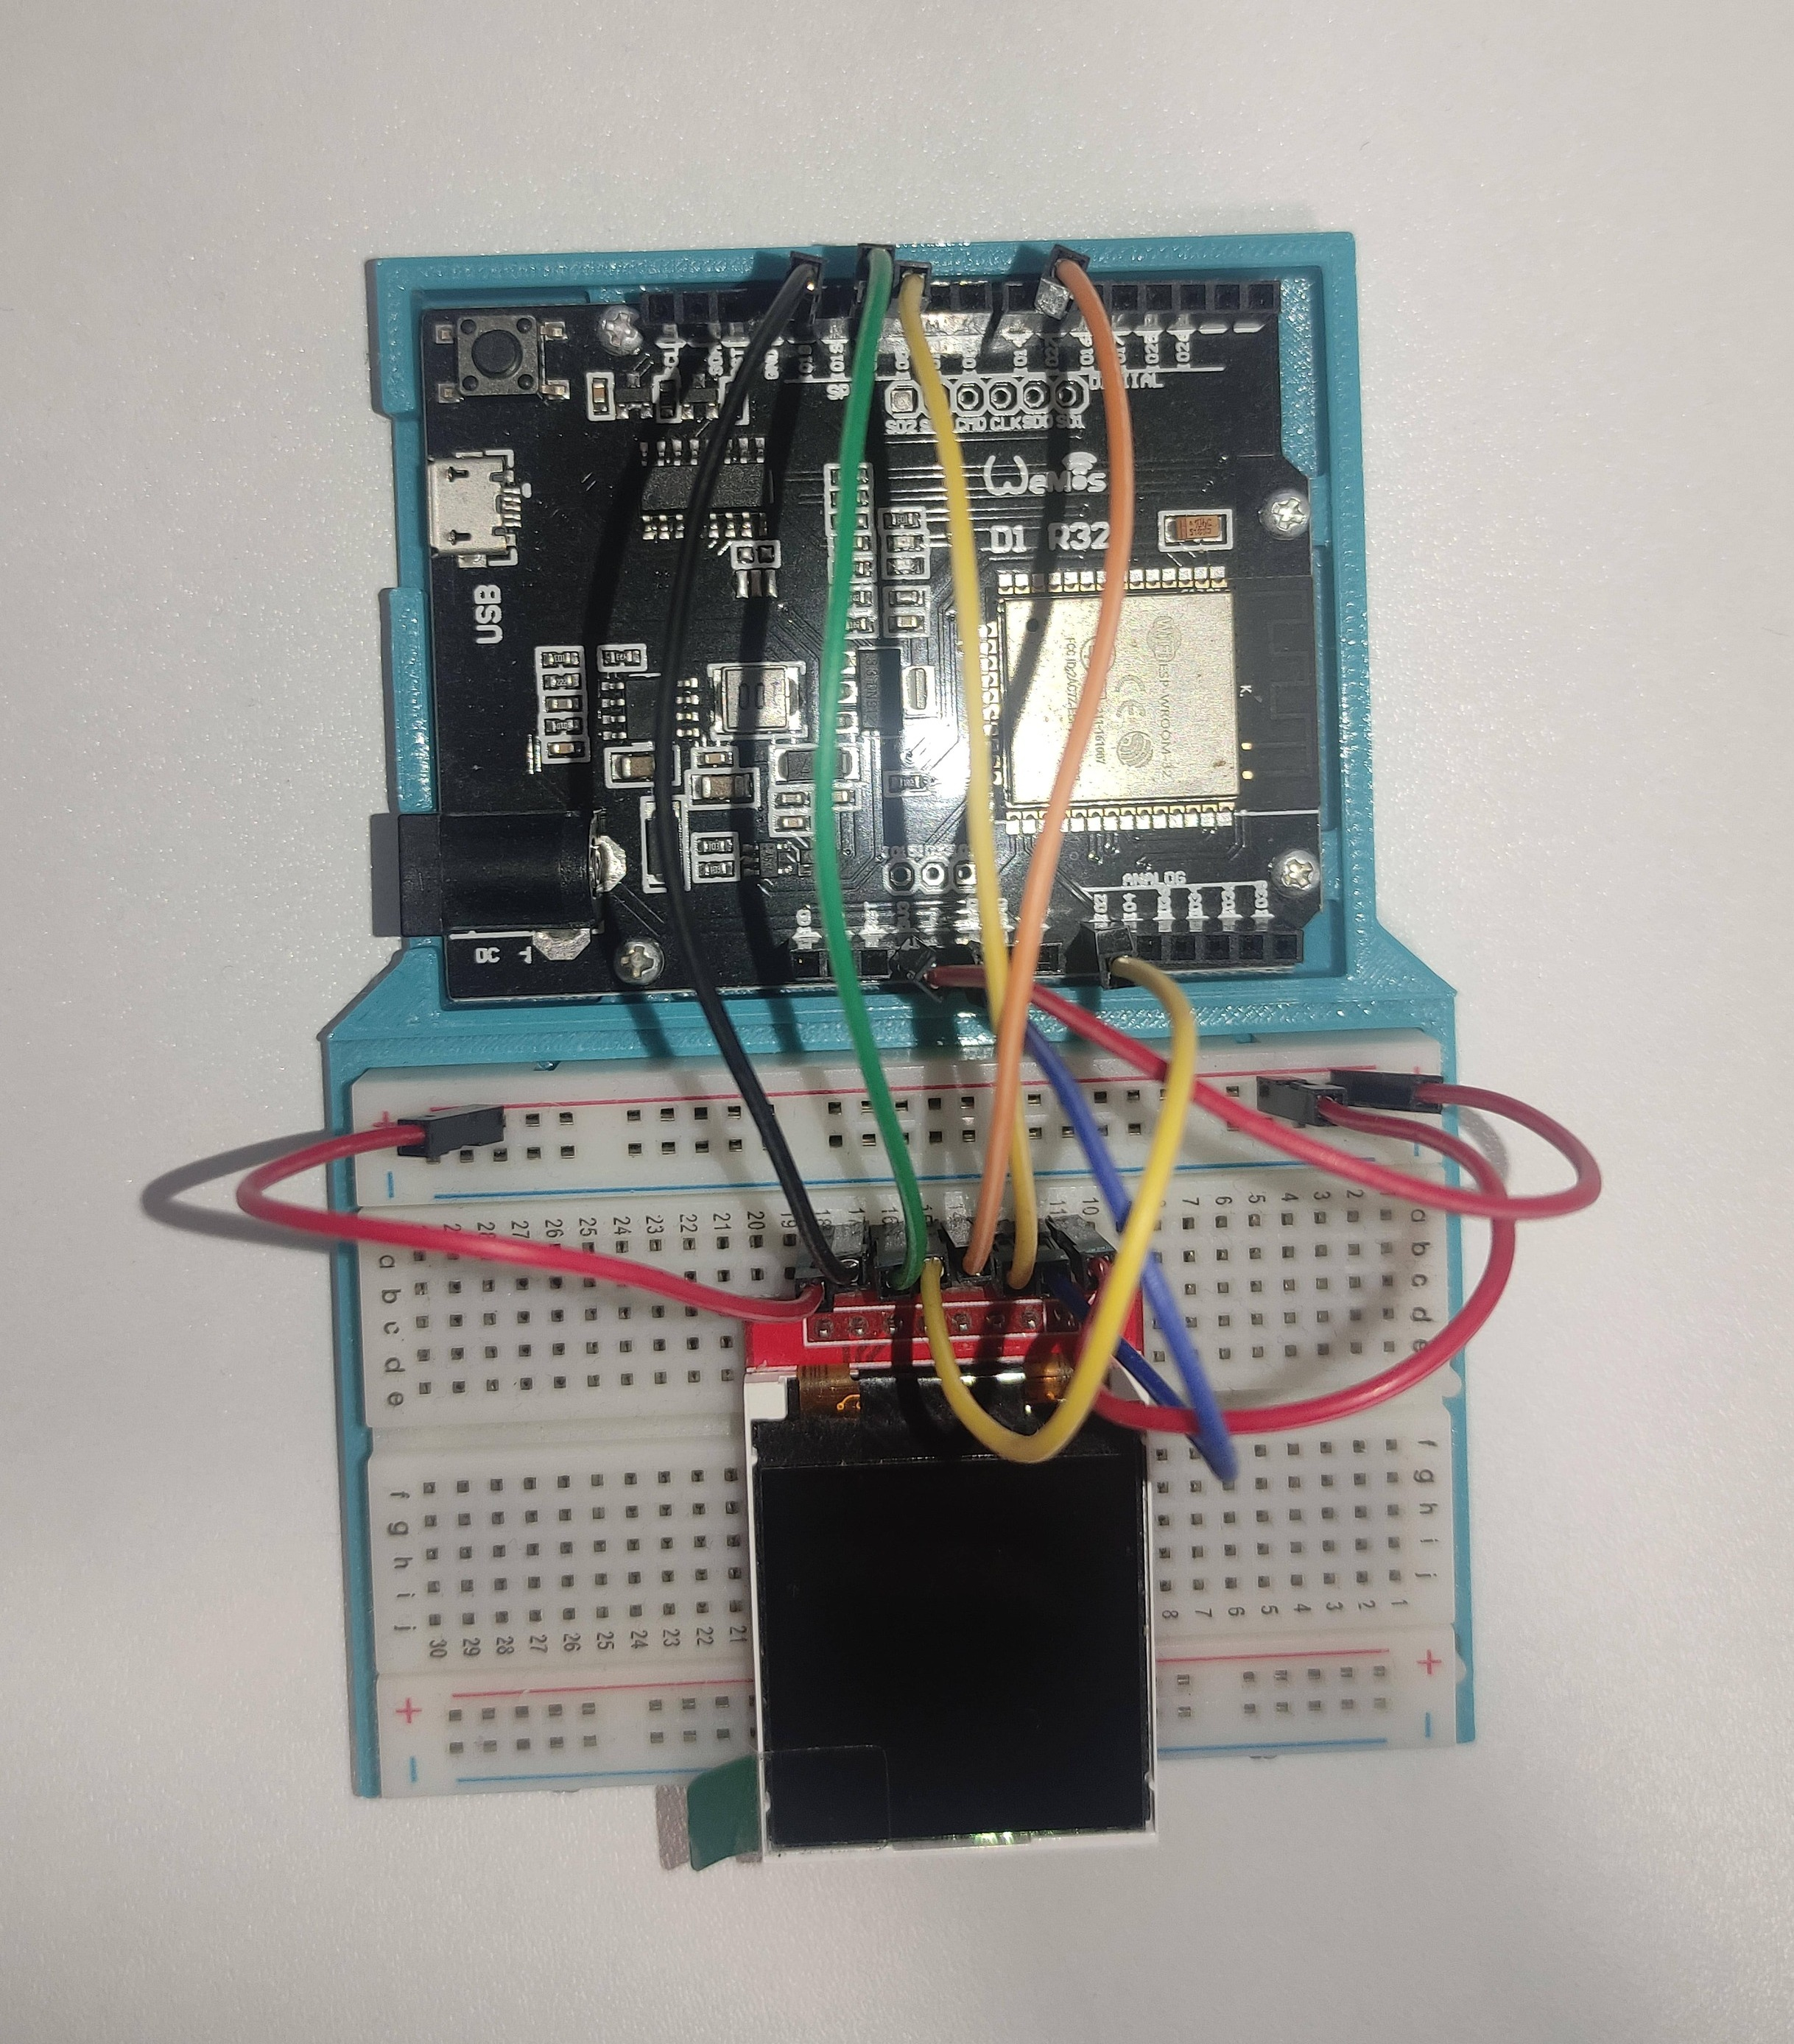
\includegraphics[width=0.7\linewidth]{obrazky-figures/wiring.jpg}
    \caption{Zobrazení zapojení TFT displeje k~vývojovému kitu ESP32.}
    \label{fig:zapojeni}
\end{figure}

\section{Vývojové prostředí}

Vývoj programu se uskutečnil v~aplikaci \texttt{vscode} s~rozšířením \texttt{PlatformIO}, které bez problému automaticky nalezlo připojený vývojový kit a nahrálo do něj nový program. Veškerý vývoj probíhal v~Linuxovém prostředí na operačním systému Ubuntu 24.04.1 LTS.

V~tomto projektu je použit Arduino framework z~důvodu kompatibility s~externími knihovnami a z~důvodu použití programovacího jazyka C++, ve kterém je následně implementovaný program. Konkrétní části programu využívají prostředků jazyka C++ jako jsou například třídy.

\chapter{Vlastnosti programu}

Program je rozdělen na 3 hlavní funkcionality. V~první pouze vykreslí text, který obdržel přes Bluetooth, na TFT displej. Toho je docíleno za pomoci metody \texttt{print} z~externí knihovny \textit{Adafruit GFX}.

Druhá funkcionalita je vykreslení obrázku. Tento obrázek se posílá po několika částech z~důvodu přetečení zásobníku pro přijatá data skrz Bluetooth komunikaci. Pokud by zásobník přetekl, některá data by se ztratila a obrázek by vypadal jinak, než by bylo očekáváno. Vykreslení obrázků je nejjemnější možné, takže lze změnit barvu každého pixelu displeje, a to až na 65 tisíc různých barev, protože se využívá dvou bajtů barvy ve formátu RGB565.

Poslední hlavní funkcionalita je hra Tetris, která se spouští, jakmile vývojový kit detekuje zmáčknutí tlačítka doleva nebo doprava. Následně lze pohybovat s~padajícími tvary pomocí těchto šipek. Pokud uživatel prohraje, obarví se mu rámeček okolo celého displeje červeně a hra se pozastaví. Z~tohoto pozastaveného bodu a vlastně kdykoliv během hry se dá odejít pomocí přijetí dalších dat, které mají buďto zobrazit obrázek, nebo vykreslit text.

Obě strany komunikace musí mít stejně definovaný tvar bajtů, které mezi sebou přenáší. V~tomto případě je tato informace v~tabulce \ref{tab:bajty}. Vývojový kit se na základě prvního bajtu celé zprávy rozhodne, zda má vypsat text, vykreslit obrázek nebo spustit hru Tetris.

\begin{table}[h!]
    \centering
    \begin{tabular}{|l|p{46mm}|p{50mm}|}
        \hline
        \textbf{Příkaz v~aplikaci}  & \textbf{Formát odesílaných dat}       & \textbf{Popisek} \\
        \hline
        Obrázek (1. část)           & 0x00 \uv{data obrázku}                & 0x00 bajt na začátku dat určuje informaci, že se bude nahrávat nový obrázek. \\
        \hline
        Obrázek (ostatní části)     & 0x01 \uv{data obrázku}                & 0x01 bajt na začátku dat určuje informaci, že obrázek má i další část. \\
        \hline
        Text                        & 0x02 \uv{text ze vstupuního pole}     & 0x02 bajt na začátku dat určuje informaci, že tato data jsou text. \\
        \hline
        Tlačítko s~levou šipkou     & 0x03                                  & Přijme pouze jeden bajt, a to 0x03. \\
        \hline
        Tlačítko s~pravou šipkou    & 0x04                                  & Přijme pouze jeden bajt, a to 0x04. \\
        \hline
    \end{tabular}
    \caption{Jednotlivé zprávy v~bajtech pro komunikaci mezi vývojovým kitem a testovací aplikací \cite{AppPixelBluetoothCanvas}.}
    \label{tab:bajty}
\end{table}

\section{Testování}
\label{sec:test}

Testování probíhalo skrze aplikaci \cite{AppPixelBluetoothCanvas}, která posílá data ve správném formátu přes Bluetooth na výukový kit ESP32. Tato aplikace se pomocí Bluetooth adresy vývojového kitu s~ním spáruje a poté na něj odesílá data. Nejdříve zpracovává nakreslený obraz, napsaný text nebo zmáčknuté tlačítko do bajtových instrukcí, které se poté pošlou na ESP32 a vývojový kit následně podle prvního bajtu určí následující sekvenci instrukcí, která se provede.

Z~testů bylo zjištěno, že Bluetooth má zásobník ne přijatá data a pokud dostane příliš moc dat, nebo je dostává rychleji než zpracovává, může dojít k~přetečení a ke ztrátě dat. Toto se výrazně projevuje u~obrázku, tudíž jsou tyto obrázky posílány po částech, kde program nejdříve zpracuje první část a až po nějaké chvilce mu přijdou data na druhou část. Z~většiny toto vyřešilo zmíněný problém, avšak někdy se data stejně ztratí. V~tomto případě je doporučeno proces opakovat a nahrát obrázek znovu.

\chapter{Závěr}

Program ve spojení s~aplikací \cite{AppPixelBluetoothCanvas} funguje skvěle a zvládne zobrazit text, či nakreslený obrázek. Všechna data se mezi počítačem a vývojovým kitem ESP32 odesílají pomocí Bluetooth a poté skrze SPI rozhraní zobrazují na TFT displeji.

Program by se určitě dal vylepšit minimálně ze strany Tetrisu o~chybějící rotace tvarů. Ačkoliv je implementováno odebírání zaplněné řady a posunutí všech čtverečků nad touto řadou, nelze to jednoduše dokázat a obecně hraní Tetrisu bez možnosti otočit právě padající dílek není úplně příjemné.

\section*{Výsledek autoevaluace}

Zadání vyžaduje autoevaluaci vlastního projektu a to je zobrazeno níže v~tabulce \ref{tab:autoevaluace}.

\begin{table}[h!]
    \centering
    \begin{tabular}{|l|p{62mm}|c|}
        \hline
        \textbf{Položka} & \textbf{Popis hodnocení} & \textbf{Očekávané body} \\
        \hline
        E (Přístup k~řešení)     & Dostatečný zájem k~řešení projektu s~implementováním Tetrisu nad rámec zadání. & 2/2 \\
        \hline
        F (Funkčnost řešení)     & Funkčnost zadání splněna. & 5/5 \\
        \hline
        Q (Kvalita řešení)       & Splňuje všechno potřebné ze zadání s~menším nedostatkem, a to použitím Arduino frameworku. & 1/2 \\
        \hline
        P (Prezentace)           & Video ukazuje všechno potřebné včetně složitějšího zaplnění řady v~Tetrise a jejího následného smazání se zhoršenou kvalitou. & 1,5/2 \\
        \hline
        D (Dokumentace k~řešení) & Dokumentace má samozřejmě svoje chyby, ale základní struktura je dostatečně splněna. & 2,5/3 \\
        \hline
    \end{tabular}
    \caption{Autoevaluace projektu podle hodnoticího klíče z~\cite{HodnoticiKlic}.}
    \label{tab:autoevaluace}
\end{table}
